\renewcommand{\figurename}{}
\mychapter{R3.14 Mathématiques: Analyse de Fourier (27h)}{cap:r314} 
\lhead{R3.14 Mathématiques: Analyse de Fourier (27h)}

\vspace*{0.2cm}%
      \large
      \href{}{\color{black}Enseignant\\Sophie Métatidj}\\%
      \normalsize
\vspace*{0.5cm}%

Unique module de mathématiques de cette deuxième année, consacré aux séries et aux transformés de Fourier. Son objectif lors de cette deuxième période était de nous familiariser avec la décomposition de signaux périodiques en sommes de sinusoïdes, et de pouvoir correctement les manipuler pour la suite.
\\ \\
Chaque signal périodique peut être représenté sous la forme d'une somme infinie de sinusoïdes simples (une fréquence) par M. Fourier. Plusieurs théorèmes en découlent comme celui de Dirichlet étudié, indiquant qu'en tout point d'un signal périodique, le point pris sera développable en une série de Fourier (en discontinuité aussi, donc pas de point).
\\ \\
Nous avons vu lors des travaux d'intégration la compréhension des sommes de sinusoïdes et comment les caractériser. En caractérisant les harmoniques d'un signal (paires, impaires selon les signaux périodiques), les aires des périodes et les calculs de série de Fourier en un point défini.

\begin{figure}[H]
    \centering
    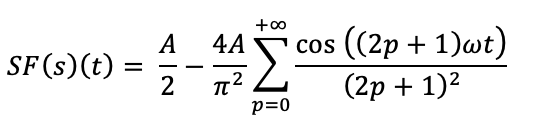
\includegraphics[width=\textwidth - \textwidth / 2]{ressources/r314/00.png}
    \caption{Exemple d'expression d'une expression en série de Fourier SF.}
    \label{fig:r314-00}
\end{figure}

Nous avons aussi caractérisé mathématiquement un signal périodique par le biai de questions pour nous familiariser avec la décomposition en série.

\begin{figure}[H]
    \centering
    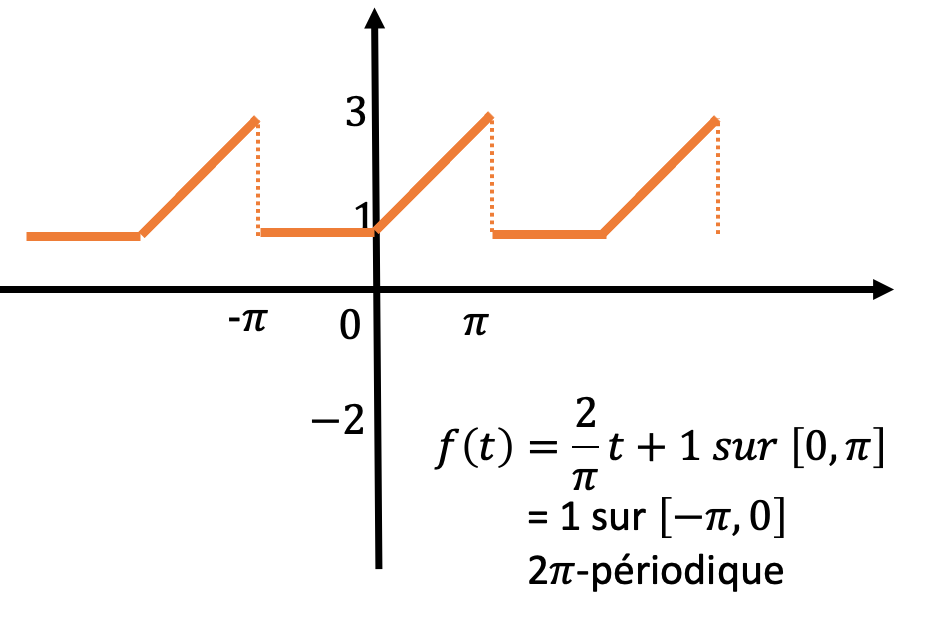
\includegraphics[width=\textwidth - \textwidth / 3]{ressources/r314/01.png}
    \caption{Exemple d'un signal donné à étudié, étude guidé par un enchainement de questions.}
    \label{fig:r314-01}
\end{figure}

L'objectif de cette première période était aussi de nous préparer à ce que nous allions comprendre sous le nom de transformées de Fourier TF, nous avons uniquement vu cette période les séries de Fourier SF.